\section{Kiểm thử Hệ thống}

\subsection{Mục tiêu và Môi trường Kiểm thử}

Quá trình kiểm thử được thực hiện nhằm đánh giá tính đúng đắn của các chức năng quản lý thư viện, sự phối hợp giữa các tầng hệ thống, các quy trình nghiệp vụ chính và các yêu cầu về an ninh, xử lý lỗi. Phạm vi tập trung vào backend Express/TypeScript, bao gồm các mô-đun về xác thực, người dùng, sách, chi nhánh, lưu thông tài liệu và các tính năng AI.\\

\textbf{Các Công cụ Sử dụng}
\begin{itemize}
        \item Jest kết hợp với ts-jest để thực thi các ca kiểm thử TypeScript.
        \item Supertest để gửi các yêu cầu HTTP đến ứng dụng Express trong quá trình kiểm thử tích hợp và kiểm thử hệ thống.
        \item Mock Prisma Client và các dịch vụ bên ngoài giả lập cho kiểm thử cô lập, loại bỏ sự phụ thuộc vào cơ sở dữ liệu thực hoặc dịch vụ email.
        \item Trình biên dịch TypeScript với cờ \texttt{--noEmit} cùng với Jest để kiểm tra chất lượng mã nguồn.
\end{itemize}

\noindent Mã nguồn kiểm thử được tổ chức trong thư mục \texttt{backend-express/tests}, chia thành bốn danh mục: \texttt{unit}, \texttt{integration}, \texttt{system}, và \texttt{quality}. Các bài kiểm thử chạy trong môi trường Node.js và được cấu hình tập trung trong tệp \texttt{jest.config.js}.

\subsection{Kiểm thử Đơn vị (Unit Testing)}

\textbf{Mục tiêu} \\

Xác minh tính đúng đắn của từng hàm hoặc mô-đun riêng lẻ trong sự cô lập. Các ca kiểm thử tập trung vào logic nghiệp vụ, kiểm tra dữ liệu đầu vào, mã lỗi HTTP, xác thực token, xử lý mật khẩu và các nhánh ngoại lệ. Prisma Client, mailer và các phụ thuộc bên ngoài được thay thế bằng các đối tượng giả lập (mock) để kết quả không bị ảnh hưởng bởi môi trường thực thi.\\

\noindent \textbf{Phương pháp luận} \\

Mỗi hàm được kiểm thử với các trường hợp hợp lệ, không hợp lệ, biên và ngoại lệ. Các nhóm chức năng chính bao gồm đăng ký và đăng nhập, xác thực OTP, quản lý sách, quản lý độc giả, lưu thông tài liệu, middleware xác thực và chuẩn hóa lỗi.

\begin{table}[H]
\centering
\caption{Phạm vi và Kết quả Kiểm thử Đơn vị}
\begin{tabularx}{\textwidth}{|p{4.2cm}|X|c|c|}
\hline
\textbf{Nhóm Kiểm thử} & \textbf{Nội dung Chính} & \textbf{Suites} & \textbf{Kết quả} \\
\hline
Auth và DTO & Đăng ký, OTP, đăng nhập, kiểm tra dữ liệu đầu vào & 3 & Đạt (Pass) \\
\hline
Sách & CRUD sách, tiện ích sách, quản lý danh mục & 3 & Đạt (Pass) \\
\hline
Người dùng và Chi nhánh & Hồ sơ độc giả, logic nghiệp vụ chi nhánh & 2 & Đạt (Pass) \\
\hline
Lưu thông và Middleware & Mượn/trả, middleware xác thực, xử lý lỗi & 3 & Đạt (Pass) \\
\hline
\multicolumn{2}{|r|}{\textbf{Tổng cộng}} & \textbf{10} & \textbf{168/168} \\
\hline
\end{tabularx}
\end{table}

Ví dụ dưới đây kiểm thử kịch bản đăng ký với một email đã tồn tại. Kết quả kỳ vọng là dịch vụ trả về lỗi HTTP 409 và không tạo tài khoản mới.

\begin{lstlisting}[language=R, caption={Ca kiểm thử đơn vị cho tính năng đăng ký}]
it('returns 409 when email already exists', async () => {
    prismaMock.user.findUnique.mockResolvedValueOnce({ id: 'exists' });

    await expect(authService.register({
        email: 'reader@example.com',
        password: 'password1',
        fullName: 'A',
    })).rejects.toMatchObject({ statusCode: 409 });
});
\end{lstlisting}

Kết quả kiểm thử đơn vị cho thấy 10/10 bộ kiểm thử (test suites) đã vượt qua, tương ứng với 168/168 ca kiểm thử đạt. Độ bao phủ mã nguồn (code coverage) cho nhóm này đạt 94.33\% câu lệnh (statements), 77.58\% nhánh (branches), 94.44\% hàm (functions) và 95.07\% dòng (lines). \\

\begin{figure}[H]
    \centering
    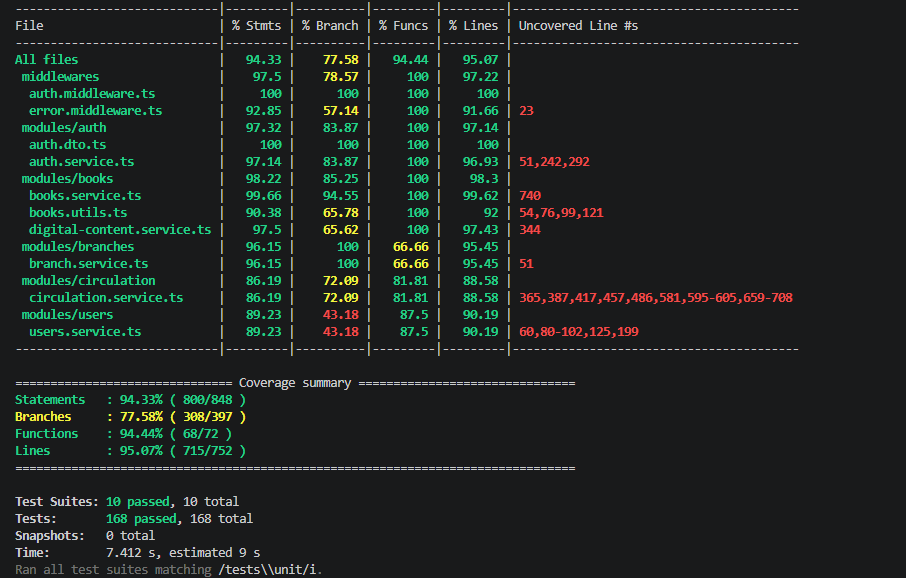
\includegraphics[width=0.9\textwidth]{Images/unit_test_result.png}
    \vspace{0.5cm}
    \caption{Kết quả kiểm thử đơn vị}
    \label{fig:unit-test-result}
\end{figure}

\subsection{Kiểm thử Tích hợp (Integration Testing)}

\textbf{Mục tiêu} \\

Xác minh sự phối hợp giữa các route, middleware, controller, service và tầng truy cập dữ liệu thông qua các yêu cầu HTTP thực tế gửi đến ứng dụng Express. Bộ kiểm thử này xác nhận cấu trúc phản hồi, mã trạng thái HTTP, cơ chế xác thực và sự tích hợp liên chức năng trong cùng mô-đun.\\

\noindent \textbf{Phương pháp luận} \\

Supertest được sử dụng để giả lập các yêu cầu GET, POST, PATCH và DELETE. Prisma Client được giả lập tại ranh giới dữ liệu, trong khi ứng dụng Express được khởi tạo đầy đủ để các route và middleware thực thi giống như trong môi trường thực.

\begin{table}[H]
\centering
\caption{Phạm vi và Kết quả Kiểm thử Tích hợp}
\begin{tabularx}{\textwidth}{|p{4.2cm}|X|c|c|}
\hline
\textbf{API/Mô-đun} & \textbf{Nội dung Kiểm thử} & \textbf{Suites} & \textbf{Kết quả} \\
\hline
Auth & Đăng ký, xác thực OTP, đăng nhập, lỗi dữ liệu đầu vào & 1 & Đạt (Pass) \\
\hline
Sách và Chi nhánh & Tra cứu sách, quản lý danh mục và chi nhánh & 2 & Đạt (Pass) \\
\hline
Người dùng và Lưu thông & Hồ sơ người dùng, mượn, trả, gia hạn & 2 & Đạt (Pass) \\
\hline
Dịch vụ AI & Tương tác với các điểm cuối dịch vụ AI & 1 & Đạt (Pass) \\
\hline
\multicolumn{2}{|r|}{\textbf{Tổng cộng}} & \textbf{6} & \textbf{67/67} \\
\hline
\end{tabularx}
\end{table}

Ví dụ dưới đây kiểm thử API đăng nhập với thông tin hợp lệ. Ngoài mã trạng thái HTTP 200, bài kiểm thử xác nhận nội dung phản hồi chứa access token, refresh token và chi tiết hồ sơ người dùng.

\begin{lstlisting}[language=R, caption={Ca kiểm thử tích hợp cho API đăng nhập}]
const response = await request(app)
    .post('/api/v1/auth/login')
    .send({ email: 'reader@library.edu.vn', password: 'CorrectPass@123' });

expect(response.status).toBe(200);
expect(response.body.success).toBe(true);
expect(response.body.data.accessToken).toBeDefined();
expect(response.body.data.refreshToken).toBeDefined();
\end{lstlisting}

Kiểm thử tích hợp đạt 6/6 bộ kiểm thử và 67/67 ca kiểm thử vượt qua. Tất cả các điểm cuối được đánh giá đều trả về mã trạng thái và nội dung phản hồi phù hợp cho cả kịch bản thành công lẫn kịch bản lỗi. \\

\begin{figure}[H]
    \centering
    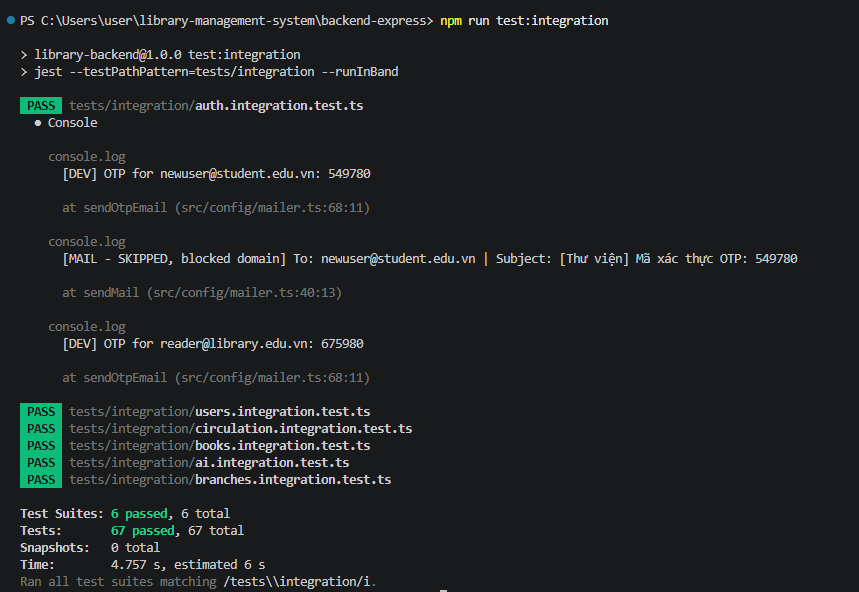
\includegraphics[width=0.9\textwidth]{Images/integration_test_result.png}
    \vspace{0.5cm}
    \caption{Kết quả kiểm thử tích hợp}
    \label{fig:integration-test-result}
\end{figure}


\subsection{Kiểm thử Hệ thống (System Testing)}

\textbf{Mục tiêu} \\ 

Xác nhận các quy trình nghiệp vụ end-to-end từ yêu cầu người dùng đến kết quả đầu ra cuối cùng của hệ thống. Nhóm này tập trung vào vòng đời độc giả, chu trình mượn--gia hạn--trả, hàng chờ đặt chỗ, tính tiền phạt quá hạn và an ninh phân quyền.\\

\noindent \textbf{Phương pháp luận}\\

Các bước nghiệp vụ được giả lập theo thứ tự tuần tự trong thực tế. Mỗi bước gửi một yêu cầu sử dụng vai trò người dùng phù hợp và xác minh cả phản hồi trả về lẫn trạng thái nghiệp vụ được cập nhật. Nhóm kiểm thử an ninh bao gồm các trường hợp biên như thiếu token, token hết hạn, token bị giả mạo, truy cập vai trò không hợp lệ, các header an ninh và điểm cuối không tồn tại.

\begin{table}[H]
\centering
\caption{Các Quy trình Kiểm thử Hệ thống}
\begin{tabularx}{\textwidth}{|p{5cm}|X|c|}
\hline
\textbf{Quy trình Nghiệp vụ} & \textbf{Nội dung Kiểm thử} & \textbf{Kết quả} \\
\hline
Vòng đời Độc giả & Đăng ký, xác thực, cập nhật hồ sơ, sử dụng tài khoản & Đạt (Pass) \\
\hline
Lưu thông Tài liệu & Thêm sách, tìm kiếm, mượn, xem lịch sử, gia hạn, trả & Đạt (Pass) \\
\hline
Đặt chỗ và Hàng chờ & Đặt chỗ tài liệu, thứ tự hàng chờ, thông báo sách về & Đạt (Pass) \\
\hline
Phạt Quá hạn & Phát hiện quá hạn, tạo khoản phạt, xử lý thanh toán & Đạt (Pass) \\
\hline
An ninh Hệ thống & JWT, RBAC, Helmet, lỗi 404, dữ liệu JSON không hợp lệ & Đạt (Pass) \\
\hline
\multicolumn{1}{|r|}{\textbf{Tổng cộng}} & \textbf{5 bộ kiểm thử, 36 ca kiểm thử} & \textbf{36/36} \\
\hline
\end{tabularx}
\end{table}

Ví dụ, quy trình lưu thông lần lượt kiểm tra việc thủ thư thêm sách, độc giả tìm kiếm sách, thủ thư tạo phiếu mượn và độc giả yêu cầu gia hạn. Ca kiểm thử dưới đây xác minh vai trò thủ thư được cấp quyền tạo phiếu mượn:

\begin{lstlisting}[language=R, caption={Ca kiểm thử hệ thống cho quy trình mượn sách}]
const response = await request(app)
    .post('/api/v1/circulation/borrow')
    .set(roleAuthHeader(Role.LIBRARIAN, librarianId))
    .send({ userId: readerId, barcode: copyBarcode });

expect(response.status).toBe(201);
expect(response.body.success).toBe(true);
expect(response.body.data.borrowRecordId).toBe(borrowRecordId);
\end{lstlisting}

Kết quả cho thấy toàn bộ 5 quy trình hệ thống đã vượt qua, với 36/36 ca kiểm thử thành công. Các trường hợp thiếu token, token không hợp lệ, truy cập trái phép và dữ liệu JSON sai định dạng đều bị từ chối chính xác với các mã trạng thái HTTP phù hợp. \\

\begin{figure}[H]
    \centering
    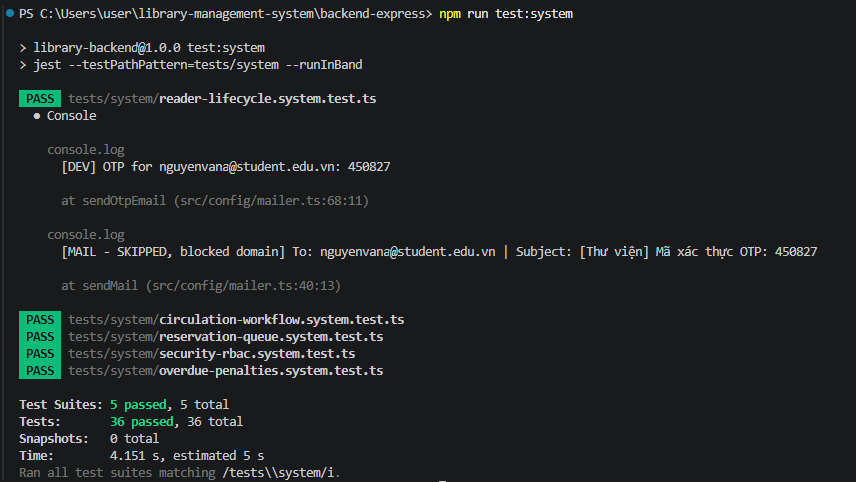
\includegraphics[width=0.9\textwidth]{Images/system_test_result.png}
    \vspace{0.5cm}
    \caption{Kết quả kiểm thử hệ thống}
    \label{fig:system-test-result}
\end{figure}

\subsection{Kiểm thử Chất lượng Mã nguồn (Code Quality Testing)}

\textbf{Mục tiêu} \\

Đánh giá các điều kiện chất lượng tĩnh và quy ước kiến trúc bên cạnh việc kiểm thử chức năng. Các chủ đề xác minh bao gồm biên dịch TypeScript, tính toàn vẹn thư mục nguồn, phát hiện secret hardcode, phân tầng route--service, cấu trúc phản hồi API và mã lỗi chuẩn hóa.\\

\noindent \textbf{Phương pháp luận} \\ 

Các bài kiểm thử phân tích các tệp TypeScript trong thư mục \texttt{src} đồng thời thực thi \texttt{npx tsc --noEmit}. Các tiêu chí được diễn đạt dưới dạng các khẳng định Jest để bất kỳ vi phạm nào cũng tự động bị bắt trong đường ống kiểm thử.

\begin{table}[H]
\centering
\caption{Kết quả Kiểm thử Chất lượng Mã nguồn}
\begin{tabularx}{\textwidth}{|p{6cm}|X|c|}
\hline
\textbf{Tiêu chí} & \textbf{Nội dung Kiểm thử} & \textbf{Kết quả} \\
\hline
Biên dịch TypeScript & Toàn bộ backend biên dịch không có lỗi kiểu & Đạt (Pass) \\
\hline
Tính Toàn vẹn Mã nguồn & Thư mục \texttt{src} tồn tại; các tệp TypeScript không rỗng & Đạt (Pass) \\
\hline
An ninh & Không có mật khẩu, secret JWT hay chuỗi kết nối hardcode & Đạt (Pass) \\
\hline
Kiến trúc Phân tầng & Route không gọi Prisma trực tiếp; controller chuyển lỗi qua \texttt{next} & Đạt (Pass) \\
\hline
Phản hồi và Mã Lỗi & Thuộc tính \texttt{success} chuẩn hóa và mã trạng thái HTTP hợp lệ & Đạt (Pass) \\
\hline
\multicolumn{1}{|r|}{\textbf{Tổng cộng}} & \textbf{2 bộ kiểm thử, 10 ca kiểm thử} & \textbf{10/10} \\
\hline
\end{tabularx}
\end{table}

\begin{figure}[H]
    \centering
    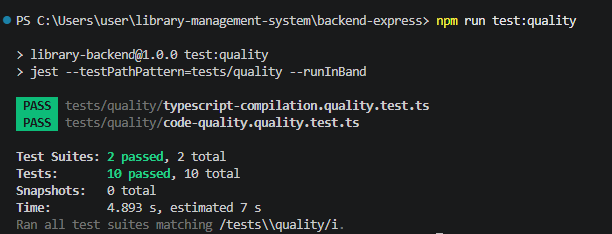
\includegraphics[width=0.9\textwidth]{Images/quality_test_result.png}
    \vspace{0.5cm}
    \caption{Kết quả kiểm thử chất lượng mã nguồn}
    \label{fig:quality-test-result}
\end{figure}

\subsection{Tổng kết Kiểm thử}

Tất cả các bài kiểm thử backend đã được thực thi bằng lệnh \texttt{npm test -- --runInBand}. Tổng hợp chung được trình bày trong Bảng~\ref{tab:test-summary}.

\begin{table}[H]
\centering
\caption{Tổng kết Kiểm thử Backend}
\label{tab:test-summary}
\begin{tabular}{|l|r|r|r|}
\hline
\textbf{Loại Kiểm thử} & \textbf{Bộ Kiểm thử (Suites)} & \textbf{Ca Kiểm thử (Cases)} & \textbf{Đạt (Passed)} \\
\hline
Kiểm thử Đơn vị (Unit) & 10 & 168 & 168 \\
\hline
Kiểm thử Tích hợp (Integration) & 6 & 67 & 67 \\
\hline
Kiểm thử Hệ thống (System) & 5 & 36 & 36 \\
\hline
Chất lượng Mã nguồn (Quality) & 2 & 10 & 10 \\
\hline
\textbf{Tổng cộng} & \textbf{23} & \textbf{281} & \textbf{281} \\
\hline
\end{tabular}
\end{table}

\noindent Toàn bộ 23 bộ kiểm thử đã thực thi thành công với 0 ca kiểm thử thất bại và không có bài kiểm thử snapshot. Các kết quả này xác nhận rằng các chức năng chính, sự phối hợp liên tầng, các quy tắc an ninh và tiêu chuẩn chất lượng mã nguồn của backend đều đáp ứng đầy đủ các yêu cầu kiểm thử tại thời điểm đánh giá. \\

\begin{figure}[H]
    \centering
    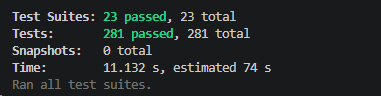
\includegraphics[width=0.9\textwidth]{Images/summary_test_result.png}
    \vspace{0.5cm}
    \caption{Tổng kết kết quả kiểm thử}
    \label{fig:summary-test-result}
\end{figure}